\documentclass[11pt]{article}
\usepackage[utf8]{inputenc}
\usepackage{titlesec}
\usepackage{titling}
\usepackage{geometry}
\usepackage{graphicx}
\usepackage{hyperref}
\usepackage{fancyhdr}
\usepackage{wallpaper}
\usepackage{afterpage} 
\usepackage{pagecolor} 
\usepackage[nottoc]{tocbibind} % Put the bibliography in the ToC
\usepackage{url}
\usepackage[toc,page]{appendix}

% Define colors
\usepackage{xcolor}
\definecolor{myblue}{RGB}{33, 66, 99}
\definecolor{mygray}{RGB}{169, 169, 169}
\definecolor{darkbluegrey}{RGB}{44, 62, 80} 

% Page styling
\pagestyle{fancy}
\fancyhf{}
\renewcommand{\headrulewidth}{0pt}
\renewcommand{\footrulewidth}{0pt}
\fancyfoot[C]{\thepage}
\renewcommand{\familydefault}{\sfdefault}

% Define a command for section headers
\titleformat{\section}
  {\color{myblue}\normalfont\Large\bfseries}
  {\color{myblue}\thesection}{1em}{}

% Define a command for subsection headers
\titleformat{\subsection}
  {\color{myblue}\normalfont\large\bfseries}
  {\color{myblue}\thesubsection}{1em}{}

% Adjust page margins
\geometry{a4paper, margin=1in}

% make references clickable
\hypersetup{
    colorlinks=true,
    linkcolor=blue,
    filecolor=magenta,      
    urlcolor=cyan,
}

\begin{document}

% Change the background color of the first page
\pagecolor{darkbluegrey}
\afterpage{\nopagecolor}

% Add a background image
\ThisCenterWallPaper{0.75}{./image/bi.png}

\begin{titlepage}
  \vspace*{\stretch{1}}
  \begin{center}
    \textcolor{white}{\textbf{\Huge Description of Work}}\\ % changed text color to white
    \vspace{1cm}
    \textcolor{white}{\Large Sound Detection and Classification\\using Spiking Neural Networks} % changed text color to white
    \vspace{3cm}
  \end{center}
  \vspace*{\stretch{2}}
  \begin{center}
    \textcolor{white}{ % changed text color to white
      \textbf{COURREGE Téo}\\
      \textbf{GANDEEL Lo'aï}\\
      \vspace{1cm}
      \Large Date: \today}
  \end{center}
  \vspace*{\stretch{1}}
\end{titlepage}

\newpage

\tableofcontents

\pagebreak

\section{Introduction}

In the constantly evolving landscape of neural network studies, the project outlined in this Description of Work (DoW) proposes to explore the field of spiking neural networks (SNNs). This effort combines both a study and a prospective implementation, with a focus on the emerging field of neuromorphic computing.

The overall goal of this project is to perform a thorough investigation and subsequent implementation of spiking neural networks. SNNs, which are inspired by the neural signaling patterns of the human brain, show promising potential in various applications, especially in real-time processing and pattern recognition.

Before getting into the specifics of our project, let us first give a brief overview of what spiking neural networks are and how they work:

A Spiking Neural Network (or SNN) is a type of artificial neural network that mimics the functionality of biological neural networks. Unlike traditional neural networks (ANNs - Artificial Neural Networks), SNNs incorporate the concept of time into their operating model. The neurons in SNNs generate spikes of activity and communicate through these spikes (like brain neurons stimulating each other with electrical impulses), allowing them to process information in a more complex and potentially more efficient manner.

This type of neural network seems to be overall less energy consuming than ANNs and potentially more efficient in terms of processing power (in practice, it will require creating an adapted hardware architecture to be able to take advantage of this potential). Therefore, it looks like the use of this type of neural network could be a viable solution to a problem of classification processing (especially in real time).


Our project focuses on a specific problem within the broader domain of audio signal processing.
When we read the survey about $SNNs^{\cite{snn_survey}}$, it was understood that training this type of model would be more difficult to train than some ANNs due to the temporal dynamics involved in SNNs. This made us want to work on a type of data that would be less computationally or ressource intensive than images or videos, which is why we decided to work on audio data. This type of data also offers the advantage of being more adaptable to pre-recorded and real-time processing.
In our case, we decided to focus our attention on the \hyperref[item:google-audioset]{Google AudioSet} database, which contains a large number of audio samples classified into different categories. This database is therefore ideal for our project, as it will allow us to train our model on a large amount of data and to test it on a large number of categories.

\subsection{Exploratory Approach - We Start from Nothing, Then Explain}

Embracing an exploratory approach, our project begins with a clean slate, seeking to understand the nuances of applying SNNs to the chosen problem. This methodological choice allows for a comprehensive examination of the feasibility and efficacy of spiking neural networks in addressing real-world challenges in audio signal processing.

The subsequent sections of this DoW will delve into the technical aspects of the project, outlining the data to be used, the chosen thematic focus, a concise review of the existing literature, and the proposed technical objectives. Additionally, considerations regarding available resources, a brief description of the final Python demonstrator, a realistic task timeline, and a curated bibliography will provide a comprehensive overview of the project's scope and ambitions.

\section{Data used}
\subsection{Choosing the type of training data}
\subsection{Feasibility (audio $>$ image - simpler)}
\subsection{Choose database}
\subsubsection{Copyright}
\subsubsection{Time for pre-processing, cleaning ...}
\subsubsection{Uncertainties about data quality, ...}
\subsection{Open to other databases}

\section{Chosen theme}
\subsection{The SNN}
\subsubsection{Definition}
Spiking Neural Network (SNN) is a variant of artificial neural network that try to mimic more closely the biological neural networks. More precisely, it tries to copy the functioning of neurons and synapses. As a result, rather than working with continually changing time values as ANNs do, SNNs work with discrete events that happen at defined times. SNNs take a set of spikes as input and produces a set of spikes as output

\begin{center}
  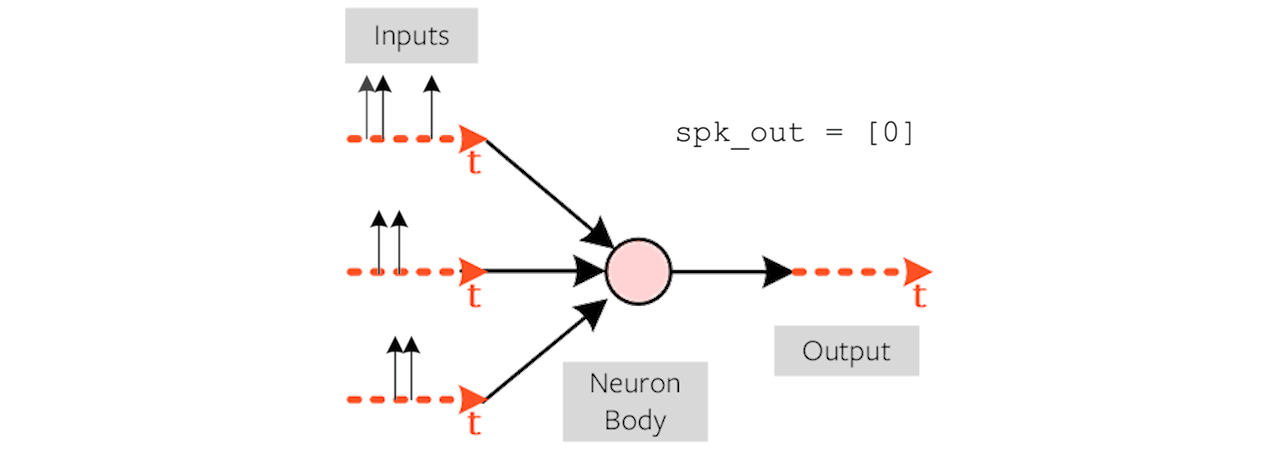
\includegraphics[scale=0.3]{image/def1.png}
  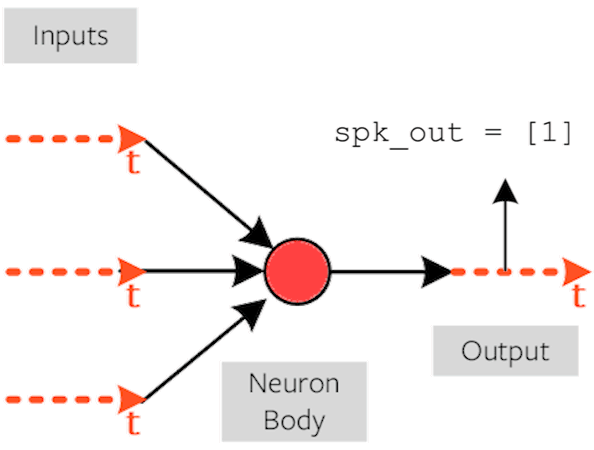
\includegraphics[scale=0.3]{image/def2.png}
\end{center}



\subsubsection{How it works}
{\color{blue}
  Key concepts

  What distinguishes a traditional ANN from a SNN is the information propagation approach.

  The general idea is as follows;

  Each neuron has a value that corresponds to the electrical potential of biological neurons at any given time.
  A neuron's value can change according to its mathematical model; for example, if a neuron receives a spike from an upstream neuron, its value can increase or decrease.
  If a neuron's value exceeds a certain threshold, the neuron will send a single impulse to each downstream neuron connected to the first, and the neuron's value will immediately drop below its average.
  As a result, the neuron goes through a refractory period similar to that of a biological neuron. The neuron's value will gradually return to its mean value over time.

  Spike Based Neural Codes

  Artificial spiking neural networks are designed to do neural computation. This necessitates that neural spiking is given meaning: the variables important to the computation must be defined in terms of the spikes with which spiking neurons communicate. A variety of neuronal information encodings have been proposed based on biological knowledge:

  Binary Coding:

  Binary coding is an all-or-nothing encoding in which a neuron is either active or inactive within a specific time interval, firing one or more spikes throughout that time frame. The finding that physiological neurons tend to activate when they receive input (a sensory stimulus such as light or external electrical inputs) encouraged this encoding.

  Individual neurons can benefit from this binary abstraction because they are portrayed as binary units that can only accept two on/off values. It can also be applied to the interpretation of spike trains from current spiking neural networks, where a binary interpretation of the output spike trains is employed in spike train classification.

  Rate Coding:

  Only the rate of spikes in an interval is employed as a metric for the information communicated in rate coding, which is an abstraction from the timed nature of spikes. The fact that physiological neurons fire more frequently for stronger (sensory or artificial) stimuli motivates rate encoding.

  It can be used at the single-neuron level or in the interpretation of spike trains once more. In the first scenario, neurons are directly described as rate neurons, which convert real-valued input numbers  “rates”  into an output “rate” at each time step. In technical contexts and cognitive research, rate coding has been the concept behind conventional artificial “sigmoidal” neurons.

  Fully Temporal Codes

  The encoding of a fully temporal code is dependent on the precise timing of all spikes. Evidence from neuroscience suggests that spike-timing can be incredibly precise and repeatable. Timings are related to a certain (internal or external) event in a fully temporal code (such as the onset of a stimulus or spike of a reference neuron).

  Latency Coding

  The timing of spikes is used in latency coding, but not the number of spikes. The latency between a specific (internal or external) event and the first spike is used to encode information. This is based on the finding that significant sensory events cause upstream neurons to spike earlier.

  This encoding has been employed in both unsupervised and supervised learning approaches, such as SpikeProp and the Chronotron, among others. Information about a stimulus is encoded in the order in which neurons within a group generate their first spikes, which is closely connected to rank-order coding.
}


\subsubsection{Advantages / Disadvantages}

{\color{blue}
  SNNs offer the following benefits

  - Energy efficiency: SNNs are highly energy efficient because they only consume energy when a spike is generated, unlike "classical" neural networks which consume energy continuously. This makes them ideal for low-power embedded devices.

  - Event-driven processing: While ANNs typically operate on a fixed time interval, SNNs only process information when there is an input spike. This makes them highly efficient at processing information in an event-driven environment, such as processing visual or auditory data.

  - Temporal coding: SNNs are able to process information based on the timing of spikes, allowing them to encode temporal information and be temporally accurate. This is particularly useful for tasks that require the processing of sequential data, such as speech or gesture recognition.

  - Robustness to noise: SNNs are inherently robust to noise and can effectively filter out irrelevant information. This makes them useful in environments where noise is a common problem, such as medical imaging or environmental monitoring.

  - Neuroplasticity: SNNs are able to adapt to new inputs and change their behaviour over time, much like the brain. This allows them to learn and adapt to new tasks and environments, making them highly versatile.


  Disadvantages:

  - SNNs are difficult to train.
  - There is currently no learning algorithm designed specifically for this task.
  - Building a small SNN is impractical.
}



\subsubsection{snnTorch}
We will primarily work in Python and use the snnTorch package to work on SNNs. snnTorch is a Python package for performing gradient-based learning with spiking neural networks. snnTorch is built on top of Pytorch and takes advantage of its GPU-accelerated tensor computation. Pre-defined spiking neuron models are integrated into the PyTorch framework and can be treated as recurrent activation units.

\subsection{Neural networks applied to audio classification}
\subsubsection{Definition}
{\color{blue}
  Audio classification is a machine learning and signal processing task that involves categorizing or labeling audio data into different predefined classes or categories. The goal is to automatically assign a label to an audio segment based on its content or characteristics. This can be useful in various applications such as speech recognition, music genre classification, environmental sound analysis, and more.

  Applications:

  Speech Recognition: Identifying spoken words or phrases in audio recordings.
  Music Genre Classification: Categorizing music into different genres, such as rock, pop, jazz, etc.
  Environmental Sound Analysis: Detecting and classifying sounds in the environment, such as sirens, footsteps, or car engines.
  Anomaly Detection: Identifying unusual or unexpected sounds in a given context.
}
\subsubsection{How it works}
{\color{blue}
  The process of audio classification typically involves the following steps

  Data collection: Collecting a dataset of audio samples, each labeled with its corresponding class or category.

  Feature extraction: Transforming the raw audio data into a set of relevant features that can be used to represent the content of the audio. Common features include spectrogram representations, Mel Frequency Cepstral Coefficients (MFCCs), and other time or frequency domain features.

  Model training: Using machine learning algorithms or deep learning architectures to train a model on the extracted features and their corresponding labels. Apart from neural networks, others algorithms can be used for audio classification such as support vector machines, decision trees, or random forests for example.

  Validation and testing: Evaluate the performance of the trained model on a separate set of data that it has not seen before. This helps evaluate the model's ability to generalize to new, unseen examples.

  Deployment: Integrate the trained model into applications or systems that require real-time or batch audio classification.
}



\subsubsection{Advantages / Disadvantages}
\subsection{Relevance of this choice}
\subsubsection{Defining the project's pros and cons}
\subsubsection{Cases of use to define the relevance of the project}

\section{State of the art}
\subsection{Finding what already exists}
\subsubsection{In a simple neural network}
\paragraph{Trained on the same data set or not}
\subsubsection{In SNN}
\paragraph{Trained on the same data set or not}
\subsubsection{Existing libraries, existing models}
\subsection{Results obtained as a basis for comparison}

\section{Technical objectives of the project}
\subsection{Technical objectives achievable with pre-existing ANNs}
\subsection{Technical objectives with data}
\subsection{Technical objectives with SNNs}
\subsection{Feasibility}
\subsubsection{Describing uncertainties}
\subsubsection{Looking for a working model}
\subsubsection{Estimate computation time}

\section{Theoretical study}
\subsection{Theoretical study on SNN}
\subsection{Investigative approach}

\section{Matching with available resources}
\subsection{Work time}
\subsection{Computer resources}
\subsection{Human resources}

\pagebreak

\section{Appendix}

\subsection{Data}

\subsubsection*{Data Set used for the project}

\begin{itemize}
  \item Google AudioSet : \url{https://research.google.com/audioset/}
  \label{item:google-audioset}
  
\end{itemize}



\subsection{Code}

\subsection{Links}

\pagebreak

% Bibliography
\bibliographystyle{siam}
\bibliography{ref}

\end{document}
